\chapter{Données et méthodologie}
\label{chapitre:methodologie}

Ce chapitre définit les données, la branche HYPO, son protocole principal de validation et
l'extension bidirectionnelle exploratoire. La sortie étudiée est une alerte comportementale
à vérifier sur le terrain. Les termes de sensibilité et de faux positif cliniques ne sont
pas employés pour la validation synthétique, faute d'étalon vétérinaire.

\section{Plan d'étude}

L'étude comporte trois niveaux. Le premier valide HYPO sur 44 événements et le compare à
trois variantes IF/LOF. Le deuxième étend la campagne à 132 scénarios pour explorer
INSTABILITÉ et cinq règles de fusion. À chaque niveau, un scénario est injecté dans une
copie distincte de la période future, puis comparé à l'exécution propre de la même
vache. Le troisième niveau est une analyse observationnelle sur une cohorte IceTag--SLS de
l'hiver 2019. Il utilise des mesures strictement antérieures au score locomoteur et ne sert
pas à régler le système. La Figure~\ref{fig:plan_etude} schématise ces trois niveaux.

\begin{figure}[H]
  \centering
  \begin{tikzpicture}[
    box/.style={rectangle, draw=black!55, rounded corners=2pt, align=center,
      minimum height=1.0cm, text width=3.0cm, inner sep=6pt, font=\small},
    arrow/.style={-{Stealth[length=2.2mm]}, thick, black!65}]
    \node[box, fill=ifblue!10] (main) {IceQube 2023\\28 vaches};
    \node[box, fill=rulegreen!10, right=0.65cm of main] (split) {Référence 60\,\%\\futur 40\,\%};
    \node[box, fill=loforange!10, right=0.65cm of split] (inject) {HYPO: 44 événements\\extension: 132 scénarios};
    \node[box, fill=profgray!10, right=0.65cm of inject] (eval) {Comparaison propre--injectée\\unité: vache};
    \draw[arrow] (main) -- (split); \draw[arrow] (split) -- (inject); \draw[arrow] (inject) -- (eval);
    \node[box, fill=ifblue!7, below=1.2cm of split] (sls) {IceTag--SLS 2019\\14 vaches};
    \node[box, fill=rulegreen!7, right=0.65cm of sls] (pre) {Sept jours\\avant le SLS};
    \node[box, fill=profgray!7, right=0.65cm of pre] (conc) {Concordance exploratoire\\sans réglage};
    \draw[arrow] (sls) -- (pre); \draw[arrow] (pre) -- (conc);
  \end{tikzpicture}
  \caption{Plan d'étude.}
  \label{fig:plan_etude}
\end{figure}

\section{Corpus principal IceQube 2023}
\label{sec:donnees}

Le fichier \texttt{data/brut.csv} provient de la ferme du campus Macdonald de
l'Université McGill. Il contient 37\,839 mesures de 28 vaches entre le
1\textsuperscript{er} octobre et le 11 novembre 2023. Les variables sont agrégées à une
résolution nominale de quinze minutes. Le Tableau~\ref{tab:dataset} en décrit les
caractéristiques vérifiées.

\begin{table}[H]
  \centering
  \caption{Caractéristiques vérifiées du corpus IceQube 2023.}
  \label{tab:dataset}
  \begin{tabular}{lr}
    \toprule
    Caractéristique & Valeur \\
    \midrule
    Vaches & 28 \\
    Lignes & 37\,839 \\
    Résolution nominale & 15 minutes \\
    Période & 1 octobre--11 novembre 2023 \\
    Lignes par vache, médiane & 564 \\
    Lignes par vache, étendue & 244--2\,474 \\
    Doublons vache--temps & 0 \\
    \bottomrule
  \end{tabular}
\end{table}

\subsection{Variables disponibles}

Les variables utilisées sont les pas, le \textit{Motion Index}, le temps couché, le temps
debout, les transitions et leur décomposition en levers et couchers
(Tableau~\ref{tab:variables_brutes}). Elles décrivent la quantité de mouvement et la
posture~; elles ne mesurent ni l'asymétrie de démarche, ni la douleur, ni une lésion du
pied \citep{alsaaod2019automatic,oleary2020accelerometers}. Leur portée clinique est donc
indirecte.

\begin{table}[H]
  \centering
  \caption{Variables brutes du corpus IceQube 2023.}
  \label{tab:variables_brutes}
  \begin{tabular}{p{0.28\textwidth}p{0.60\textwidth}}
    \toprule
    Variable & Interprétation \\
    \midrule
    \textit{Steps} & Nombre de pas dans l'intervalle. \\
    \textit{Motion Index} & Intensité agrégée du mouvement mesuré par le capteur. \\
    \textit{Lying Time} & Temps couché dans l'intervalle. \\
    \textit{Standing Time} & Temps debout dans l'intervalle. \\
    \textit{Transitions} & Nombre total de transitions posturales. \\
    \textit{Transitions Up/Down} & Décomposition en levers et couchers. \\
    \bottomrule
  \end{tabular}
\end{table}

\subsection{Statistiques descriptives et variabilité inter-individuelle}

Les distributions sont fortement asymétriques (Tableau~\ref{tab:statistiques_brutes})~: la
médiane des pas et des transitions par intervalle est nulle, tandis que les maxima sont
élevés. Cette structure écarte une normalisation gaussienne globale et motive des
comparaisons robustes propres à chaque vache et à chaque créneau horaire
\citep{leys2013detecting}.

\begin{table}[H]
  \centering
  \caption{Statistiques descriptives des variables de mouvement (par intervalle de 15~min).}
  \label{tab:statistiques_brutes}
  \begin{tabular}{lrrrr}
    \toprule
    Variable & Moyenne & Écart-type & Médiane & Maximum \\
    \midrule
    Pas & 4,0 & 15,4 & 0 & 387 \\
    \textit{Motion Index} & 25,5 & 103,7 & 5 & 3\,351 \\
    Transitions & 0,16 & 0,40 & 0 & 6 \\
    \bottomrule
  \end{tabular}
\end{table}

La variabilité entre vaches est considérable (Tableau~\ref{tab:variabilite}). La moyenne de
pas par intervalle varie de 0,0 à 11,1 selon l'animal, et le coefficient de variation
inter-vache atteint 0,50 pour les pas, 0,40 pour le \textit{Motion Index} et 0,41 pour les
transitions. Cette hétérogénéité interdit un seuil commun à tout le troupeau et justifie le
recours à une référence \emph{individuelle}, propre à chaque vache.

\begin{table}[H]
  \centering
  \caption{Variabilité inter-individuelle des principales variables (moyenne par vache).}
  \label{tab:variabilite}
  \begin{tabular}{lrrr}
    \toprule
    Variable & Moyenne/vache min & Moyenne/vache max & CV inter-vache \\
    \midrule
    Pas & 0,0 & 11,1 & 0,50 \\
    \textit{Motion Index} & 4,0 & 57,4 & 0,40 \\
    Transitions & 0,00 & 0,31 & 0,41 \\
    \bottomrule
  \end{tabular}
\end{table}

\subsection{Choix de la résolution temporelle}

L'agrégation à quinze minutes est conservée comme résolution nominale. Une résolution plus
fine multiplie le bruit et les intervalles vides sans ajouter d'information comportementale
exploitable à l'échelle d'un épisode de plusieurs heures~; une résolution plus grossière
masque les transitions posturales. Quinze minutes offrent un compromis entre stabilité du
signal et granularité suffisante pour la persistance recherchée par les deux branches.

\subsection{Contrôles d'intégrité et admissibilité}

Le chargement impose des dates interprétables, des identifiants non vides et des variables
numériques non négatives~; les durées posturales sont converties en minutes et la couverture
de chaque intervalle est conservée. Les données originales ne sont jamais modifiées par la
validation~: chaque injection opère sur une copie en mémoire.

La durée des séries est bimodale~: seize vaches possèdent moins de quatorze jours de mesures
et douze une série longue. Une vache est admissible à la validation synthétique si sa durée
atteint quatorze jours, si une période future existe après la période de référence et si les pas, le
\textit{Motion Index} et les transitions y sont informatifs. Onze vaches satisfont ces
conditions~; les 28 restent utilisables dans l'interface, l'effectif de onze ne concernant
que le protocole expérimental. La Figure~\ref{fig:admissibilite} montre la durée disponible
par vache et distingue les onze vaches admissibles, en vert, des dix-sept autres, en gris~;
le trait pointillé marque le seuil de quatorze jours. Seize des vaches grises restent sous ce
seuil, faute d'une durée suffisante. Une barre grise le dépasse pourtant~: cette
vache atteint la durée requise, mais ne fournit pas de signaux informatifs dans sa période
future, ce qui ramène l'effectif admissible à onze.

\begin{figure}[H]
  \centering
  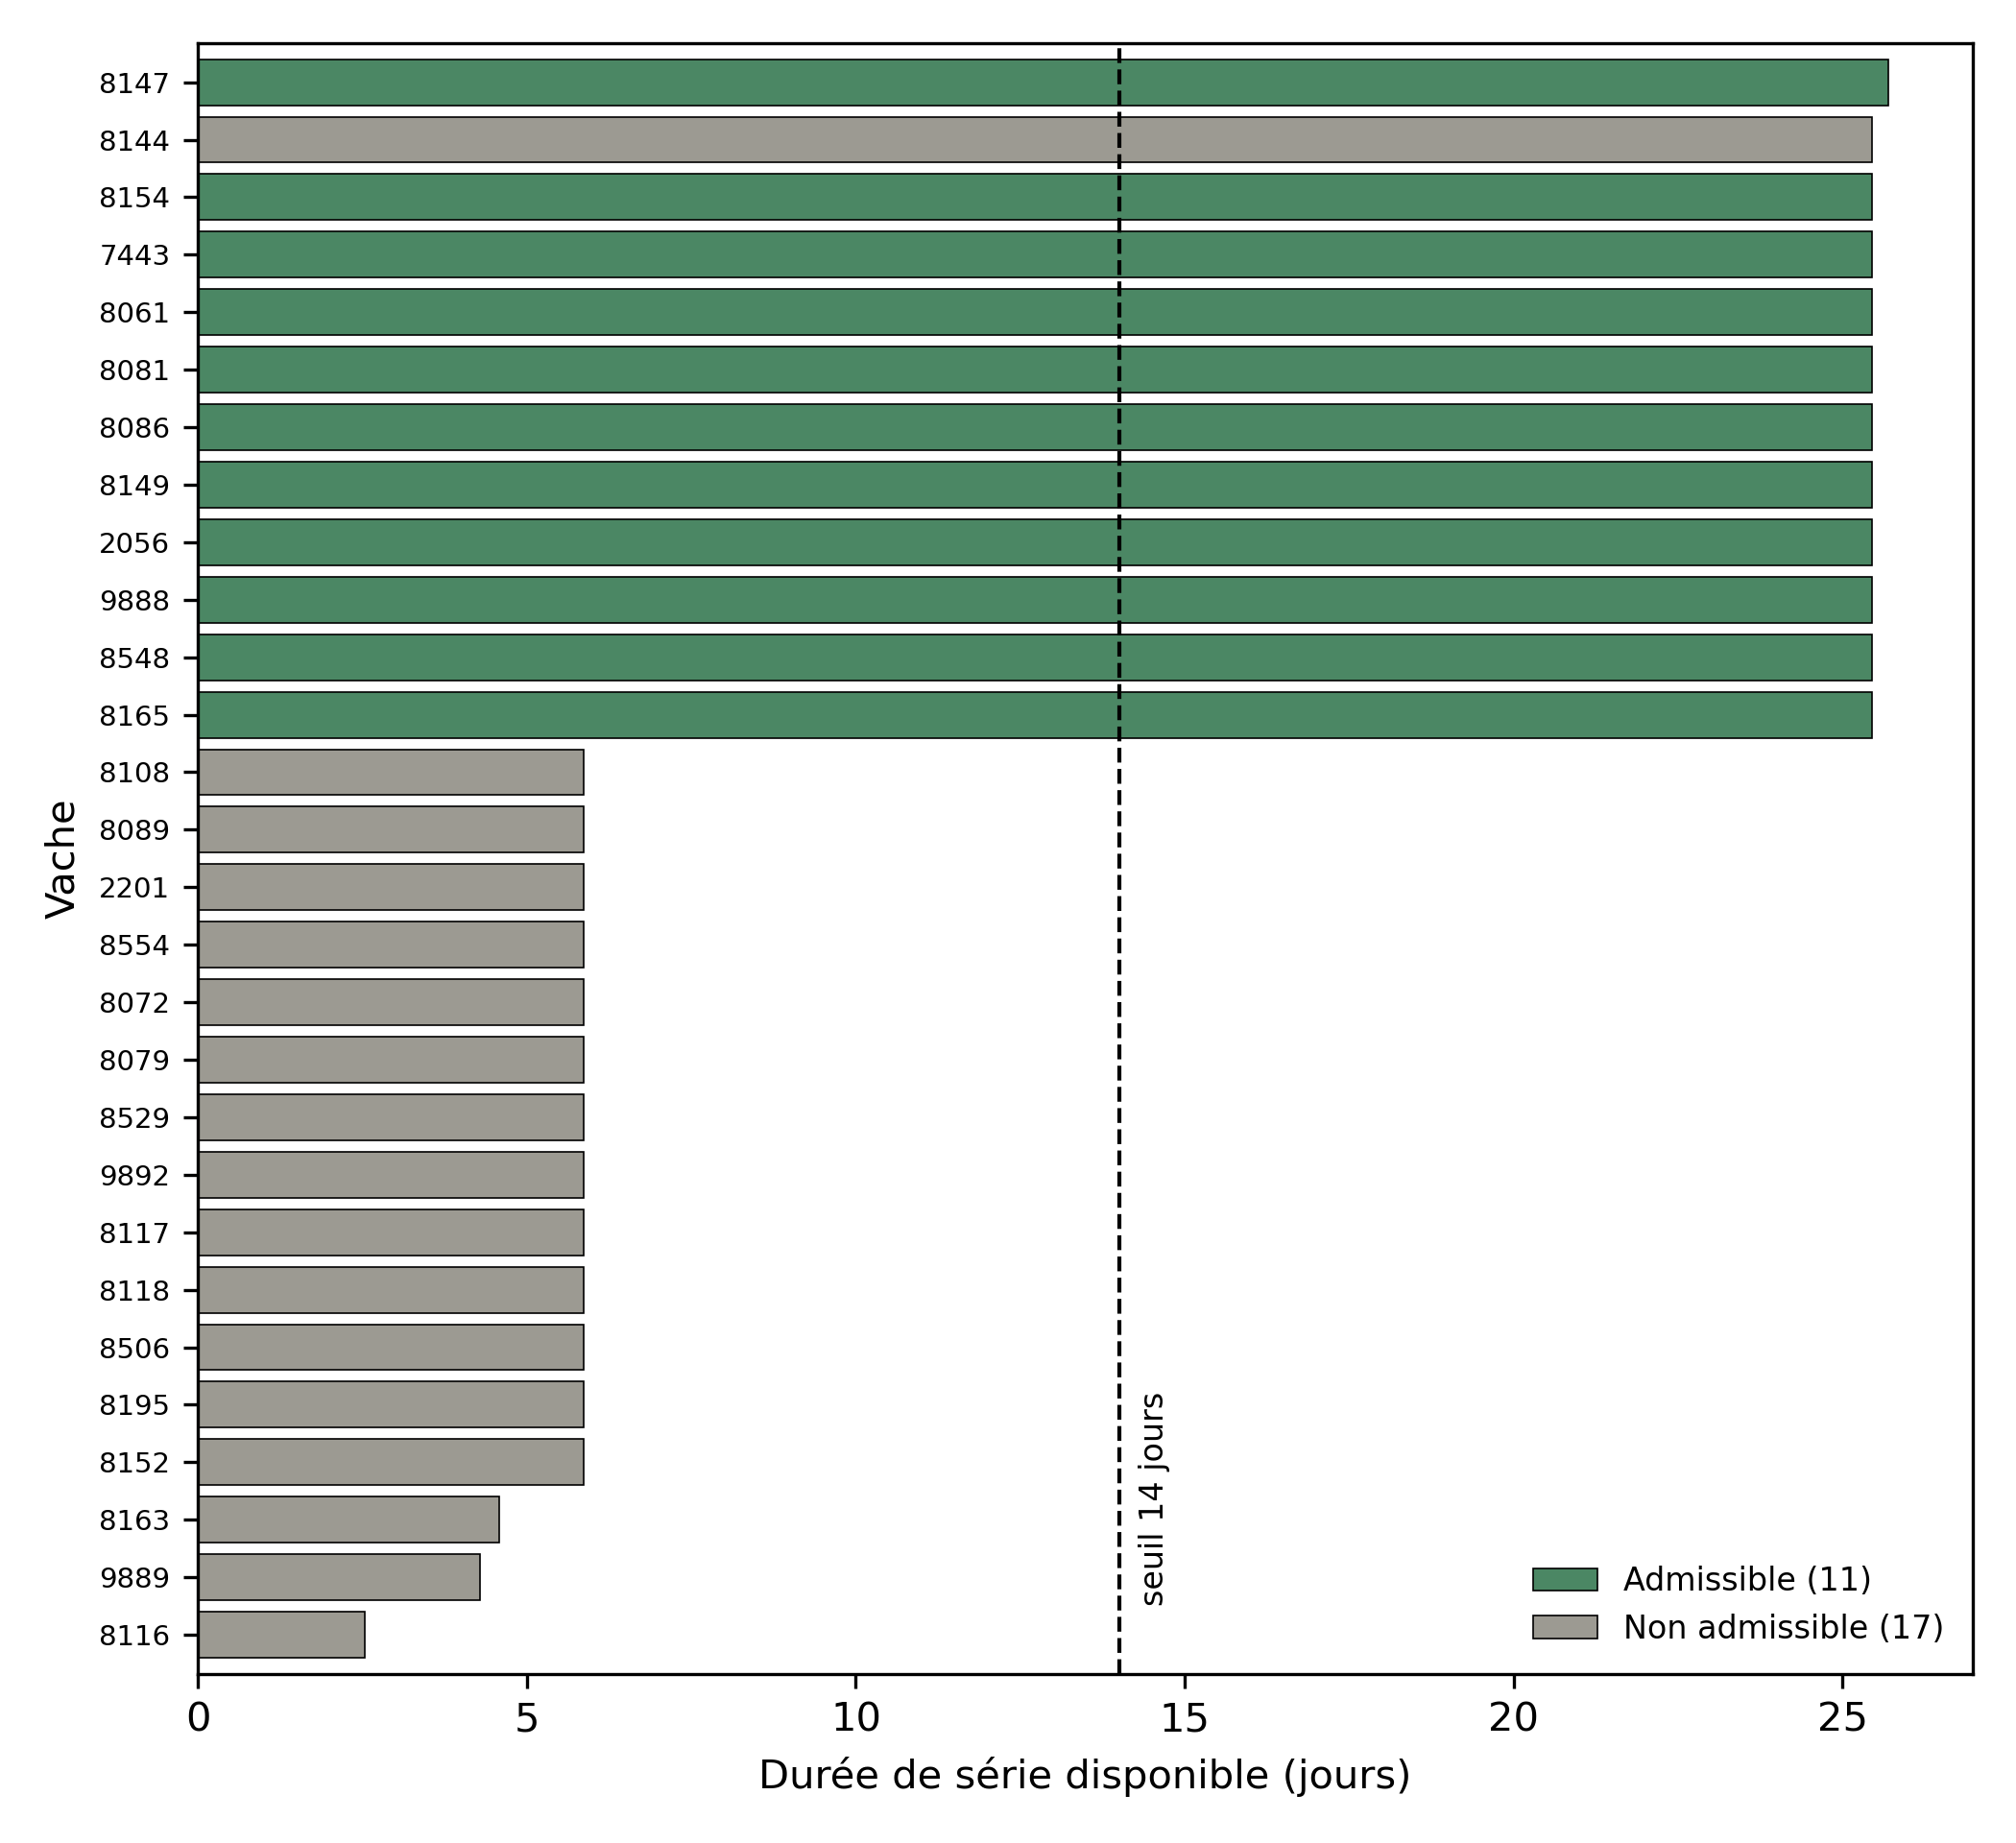
\includegraphics[width=0.80\textwidth]{figures/cow_admissibility.png}
  \caption{Admissibilité des vaches.}
  \label{fig:admissibilite}
\end{figure}

\subsection{Traçabilité et provenance des données}

La provenance du corpus a été vérifiée en confrontant ses valeurs à celles du système
commercial CowAlert (IceRobotics), qui restitue les mêmes mesures IceQube. Pour les cinq
vaches dont les mesures ont pu être relevées depuis ce système, les deux sources sont
alignées un à un sur le couple (vache, début d'intervalle), après vérification de l'absence
de doublons. Sur les 7\,631 intervalles communs parmi 7\,823 lignes CowAlert (97,5\,\%), les
pas, le \textit{Motion Index} et les transitions \emph{coïncident exactement} (corrélation de
1,0, valeurs identiques). Le corpus reflète donc les mesures restituées par le système
officiel pour ces animaux. Cette vérification porte sur cinq des vingt-huit vaches~; le
fichier source est confidentiel et n'est pas diffusé, seules les corrélations agrégées étant
rapportées.

\subsection{Variables dérivées}

Pour chaque variable brute, la chaîne de traitement construit une famille de variables dérivées
(Tableau~\ref{tab:features})~: des agrégats par intervalle, leurs transformations
logarithmiques pour atténuer l'asymétrie, un z-score robuste global et un z-score robuste
glissant (centrage par la médiane, échelle par l'écart absolu médian) et un indicateur de
couverture. Ces variables
alimentent principalement les comparateurs Isolation~Forest et Local~Outlier~Factor ainsi que
les règles de cohérence~; les deux branches temporelles, elles, raisonnent directement sur
des ratios à la référence individuelle.

\begin{table}[H]
  \centering
  \caption{Familles de variables dérivées par variable comportementale brute.}
  \label{tab:features}
  \small
  \begin{tabular}{p{0.32\textwidth}p{0.56\textwidth}}
    \toprule
    Famille & Description \\
    \midrule
    Agrégats & Somme et moyenne par intervalle de quinze minutes. \\
    Transformations log & $\log(1+x)$ sur la somme et la moyenne. \\
    Z-score robuste global & Centrage par la médiane, échelle par l'écart absolu médian (MAD). \\
    Z-score robuste glissant & Même principe sur une fenêtre mobile de 24~intervalles. \\
    Couverture & Rapport entre échantillons observés et attendus par intervalle. \\
    \bottomrule
  \end{tabular}
\end{table}

\section{Cohorte IceTag--SLS de l'hiver 2019}
\label{subsec:corpus_mcgill}

Cette cohorte provient du même campus, mais d'une période et d'un dispositif différents.
Le SLS est la somme de quatre composantes binaires et varie de 0 à 4. L'analyse retient le
score du 12 mars 2019 et les données capteurs strictement antérieures. Une vache doit avoir
une période de référence suffisante et au moins 70\,\% de couverture dans les sept jours précédents.
Quatorze vaches sont évaluables: deux ont un SLS de 0, neuf un SLS de 1 et trois un SLS de 2.
Aucun SLS de 3 ou 4 n'est observé. Le seuil SLS~$\geq2$ constitue une séparation
exploratoire, non un diagnostic imposé par le protocole source.

\section{Période de référence individuelle et contrôle de qualité}

Chaque série est triée chronologiquement. Les 60\,\% premiers intervalles admissibles
constituent la période de référence; les 40\,\% suivants forment la période future. Les médianes de
référence sont calculées pour le même créneau horaire, avec repli sur la médiane globale de
la vache. Une deuxième référence est la valeur du jour précédent. Selon le signal, la
comparaison la plus prudente entre ces deux références est retenue. Les sorties sont forcées
à zéro pendant la période de référence et un intervalle dont la couverture est inférieure à 25\,\% ne
peut devenir candidat.

\section{Branche HYPO: baisse comportementale persistante}
\label{sec:hypo}

La branche HYPO cible la signature comportementale la mieux documentée de la boiterie~: une
réduction de l'activité locomotrice (pas, mouvement, transitions) accompagnée d'une
augmentation du temps couché \citep{ito2010lying,blackie2011lying,chapinal2010measurement}.
C'est cette direction de changement, et non un écart quelconque, que le détecteur recherche.

Les pas, le \textit{Motion Index}, les transitions et les temps posturaux sont cumulés sur
douze heures. Pour les trois familles d'activité, le déficit est
\(
d_j(t)=\max(0,1-r_j(t))
\), où \(r_j(t)\) est le ratio à la référence individuelle. Le changement postural combine
l'excès de temps couché et le déficit de temps debout. Le score est
\[
S_H(t)=0{,}30d_{pas}+0{,}30d_{MI}+0{,}20d_{transitions}+0{,}20d_{posture}.
\]
Un candidat exige \(S_H\geq0{,}12\), au moins trois familles concordantes, l'implication des
pas ou du \textit{Motion Index}, une couverture suffisante et une position dans la période future.
Une baisse progressive mesurée sur six heures renforce l'évidence. Le CUSUM, somme cumulée unilatérale de Page \citep{page1954continuous}, est défini par
\(C_t=\max(0,C_{t-1}+e_t-0{,}07)\). Un épisode exige une persistance sur six heures et
\(C_t\geq1{,}20\). Deux notifications HYPO sont espacées d'au moins 24 heures. L'algorithme~\ref{alg:hypo}
résume cette logique de détection pour une vache.

\begin{figure}[H]
\centering
\fbox{\parbox{0.92\textwidth}{\raggedright
\textbf{Algorithme:} Détection HYPO d'une baisse comportementale persistante (par vache)
\vspace{0.3em}\hrule\vspace{0.5em}
\textbf{Entrée:} intervalles $X$ d'une vache, période de référence individuelle, paramètres $\theta$\\
\textbf{Sortie:} épisodes, départs et notifications (alerte à vérifier, non diagnostique)

\begin{enumerate}[leftmargin=1.5em]
\item \textit{Référence individuelle:}\\
    Pour chaque famille (pas, \textit{Motion Index}, transitions, posture), médiane de la période
    de référence par créneau horaire, avec repli sur la médiane globale de la vache.

\item \textit{Pour chaque intervalle $t$ de la période surveillée:}\\
    Totaux glissants sur $12\,$h, puis ratio $r_j(t)$ à la référence (créneau et veille, comparaison
    prudente)\\
    Déficits $d_j(t) = \max(0,\ 1 - r_j(t))$\hspace{0.5em}(posture: excès de temps couché et déficit de temps debout)\\
    Score $S_H(t) = 0{,}30\,d_{pas} + 0{,}30\,d_{MI} + 0{,}20\,d_{transitions} + 0{,}20\,d_{posture}$\\
    Candidat si $S_H \geq 0{,}12$, au moins trois familles concordantes, pas ou \textit{Motion Index}
    impliqués, et couverture suffisante\\
    Évidence $e_t \leftarrow S_H + 0{,}35\,(\text{baisse sur }6\,\text{h})$ si candidat, sinon $0$\\
    CUSUM $C_t \leftarrow \max(0,\ C_{t-1} + e_t - 0{,}07)$

\item \textit{Épisode et notification:}\\
    Épisode si persistance du candidat sur $6\,$h et $C_t \geq 1{,}20$\\
    Notifier au début d'un épisode, avec un délai réfractaire de $24\,$h
\end{enumerate}
}}
\caption{Pseudocode de la détection HYPO.}
\label{alg:hypo}
\end{figure}

La Figure~\ref{fig:hypo_cusum_example} illustre ce mécanisme sur une vache, en comparant
l'exécution injectée à l'exécution propre de la même vache.

\begin{figure}[H]
  \centering
  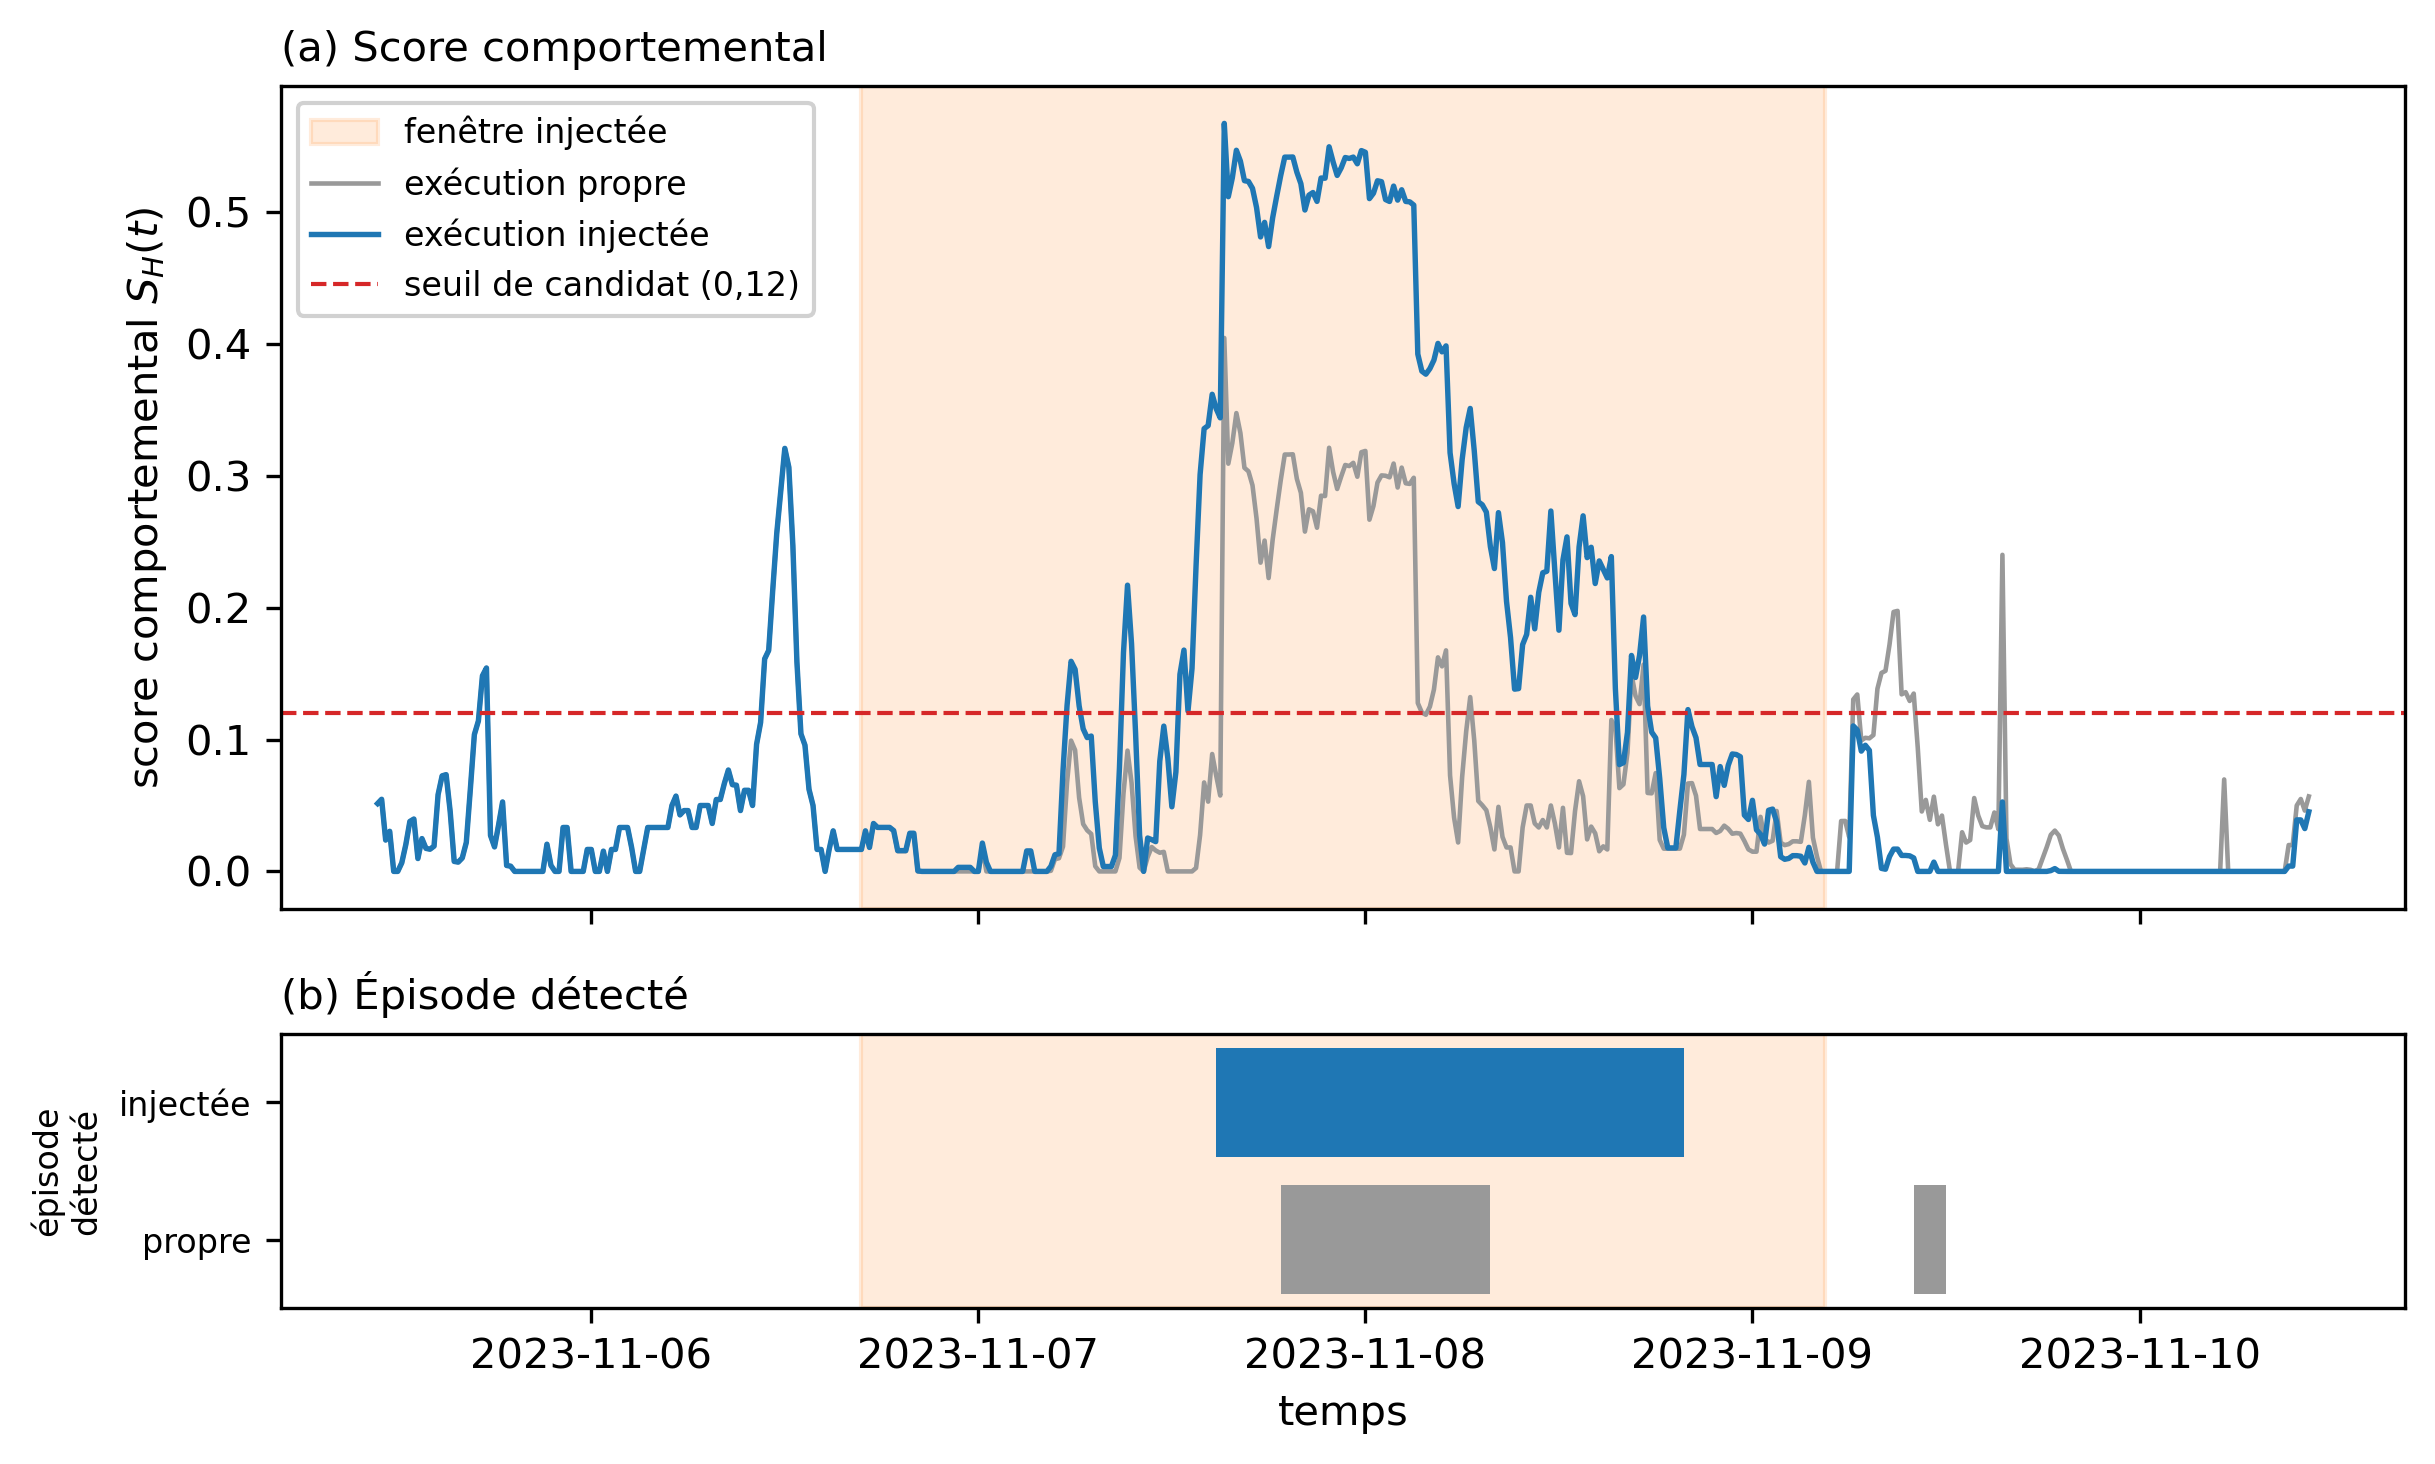
\includegraphics[width=0.95\textwidth]{figures/hypo_cusum_example.png}
  \caption[Détection attribuable au niveau de l'événement]{Détection attribuable au
  niveau de l'événement, pour une vache et une dégradation graduelle injectée après la
  période de référence. En haut, le score comportemental $S_H(t)$ de l'exécution injectée
  s'élève au-dessus du seuil de candidat et de l'exécution propre pendant la fenêtre
  injectée, puis redescend une fois l'événement terminé. En bas, l'épisode détecté de
  l'exécution injectée se superpose à la fenêtre réelle (bonne localisation temporelle),
  alors que l'exécution propre ne produit pas le même épisode au même endroit~: seule la
  part attribuable à l'injection est créditée.}
  \label{fig:hypo_cusum_example}
\end{figure}

\section{Branche INSTABILITÉ: mouvement disproportionné et posture fragmentée}
\label{sec:instabilite}

La branche INSTABILITÉ ne recherche pas une hausse globale d'activité. Elle calcule quatre
familles sur une fenêtre de trois heures: mouvement relatif aux pas, transitions relatives
aux pas, transitions relatives au temps postural et volatilité de la fraction couchée. Les
hausses des quatre familles sont pondérées respectivement par 0,35, 0,30, 0,20 et 0,15.

Un candidat exige un score d'au moins 0,18, deux familles, dont le mouvement relatif et au
moins une corroboration par transitions, fragmentation ou posture. Chaque changement
familial doit atteindre 20\,\%. Une hausse coordonnée des pas et du \textit{Motion Index}
d'au moins 15\,\%, avec un écart inférieur à 20\,\% et sans fragmentation, est filtrée comme
activité générale. Le CUSUM utilise une dérive de 0,06 et un seuil de 0,70. La persistance
est de deux heures et le délai réfractaire de douze heures.

Les paramètres de la branche INSTABILITÉ sont des choix techniques exploratoires. Ils ont
été définis avant la campagne complète puis soumis à une analyse de sensibilité. Ils ne sont
pas présentés comme des seuils physiologiques ou cliniquement optimaux.

\section{Fusion des branches}

Cinq stratégies sont comparées sur les mêmes événements:
\begin{enumerate}
  \item \textbf{HYPO}: seule la branche HYPO produit la sortie;
  \item \textbf{INSTABILITÉ}: seule l'instabilité produit la sortie;
  \item \textbf{OU}: toute branche active peut notifier;
  \item \textbf{HIÉRARCHIQUE}: l'hypoactivité, la convergence ou une séquence produit une
  alerte de vérification; l'instabilité isolée reste en surveillance;
  \item \textbf{SÉQUENTIELLE}: une alerte exige une instabilité suivie d'une hypoactivité
  entre 24 et 72 heures plus tard.
\end{enumerate}
La fusion hiérarchique est la configuration de référence de l'extension exploratoire. Sa
période réfractaire est de douze heures. Une priorité 1 correspond à une surveillance
d'instabilité, une priorité 2 à une hypoactivité et une priorité 3 à une convergence ou une
séquence. Elle n'est pas présupposée supérieure à HYPO: cette comparaison fait partie des
résultats. Le Tableau~\ref{tab:config_finale} consigne les paramètres de référence des deux
branches.

\begin{table}[H]
  \centering
  \caption{Paramètres de référence des deux branches.}
  \label{tab:config_finale}
  \small
  \begin{tabular}{lcc}
    \toprule
    Paramètre & HYPO & INSTABILITÉ \\
    \midrule
    Agrégation & 12 h & 3 h \\
    Persistance & 6 h & 2 h \\
    Délai réfractaire & 24 h & 12 h \\
    Seuil de score & 0,12 & 0,18 \\
    Dérive CUSUM & 0,07 & 0,06 \\
    Seuil CUSUM & 1,20 & 0,70 \\
    Familles minimales & 3 & 2 \\
    Couverture minimale & 25\,\% & 25\,\% \\
    \bottomrule
  \end{tabular}
\end{table}

\section{Validation technique principale du module HYPO}

Trois profils graduels et un contrôle bref sont appliqués à chacune des onze vaches
admissibles, soit 44 événements. Les profils léger, modéré et marqué diminuent de façon
progressive les pas, le mouvement et les transitions, puis transfèrent une part du temps
debout vers le temps couché pendant respectivement 36, 48 et 60 heures. Le contrôle dure
trois heures et ne devrait pas former
un épisode persistant. Chaque événement est placé dans une copie indépendante des données,
strictement après le début de la période future. L'exécution propre de la même vache est
soustraite lors du calcul des métriques attribuables.

L'ablation applique cinq variantes aux mêmes fenêtres: (A) HYPO temporel multivarié;
(B) Isolation Forest suivi des règles de persistance; (C) Isolation Forest ponctuel;
(D) LOF suivi des règles; et (E) un comparateur pédométrique restreint au seul canal des pas. Les comparaisons appariées sont calculées après agrégation par
vache. Une analyse OFAT conserve les mêmes onze vaches, les mêmes fenêtres et la même graine,
puis modifie séparément dix paramètres autour de la référence. Elle évalue une robustesse
locale et ne sélectionne pas une nouvelle configuration.

\section{Extension bidirectionnelle et contrôles de confusion}

Douze scénarios sont appliqués à chacune des onze vaches admissibles, soit 132 événements.
Chaque scénario est injecté dans une copie indépendante des données, strictement après le
début de la période future. L'enveloppe est progressive, avec montée, plateau et retour. La
somme des temps couché et debout est conservée. Le Tableau~\ref{tab:profils_v3} décrit ces
douze scénarios.

\begin{table}[H]
  \centering
  \caption{Scénarios de la validation technique.}
  \label{tab:profils_v3}
  \small
  \begin{tabular}{p{0.27\textwidth}p{0.18\textwidth}p{0.43\textwidth}}
    \toprule
    Famille & Nombre & Rôle \\
    \midrule
    Hypoactivité légère, modérée, marquée & 33 & Baisse progressive de plusieurs signaux sur 24 à 48 h. \\
    Instabilité légère, modérée, marquée & 33 & Mouvement relatif, transitions et posture sur 8 à 16 h. \\
    Instabilité puis hypoactivité & 11 & Séquence séparée par 24 h. \\
    Pic capteur, exercice bref, manipulation & 33 & Contrôles brefs qui doivent être rejetés. \\
    Activité de type œstrus & 11 & Confondant d'hyperactivité coordonnée. \\
    Hypoactivité non locomotrice & 11 & Confondant causal indiscernable avec les capteurs seuls. \\
    \bottomrule
  \end{tabular}
\end{table}

L'amplitude modérée des pas atteint 29\,\%, valeur ancrée sur un ordre de grandeur publié
autour d'un parage thérapeutique \citep{paudyal2021lying}. Les amplitudes des autres signaux
sont des hypothèses de test et non des estimations cliniques.

\section{Métriques et analyses de sensibilité}

\subsection{Recouvrement temporel (IoU)}

La localisation d'un épisode est mesurée par l'intersection sur l'union
(\textit{Intersection over Union}, IoU), une métrique issue de la détection d'objets en
vision par ordinateur \citep{everingham2010pascal}, entre la fenêtre injectée et l'épisode
prédit~:
\[
\mathrm{IoU} = \frac{|\,\text{injecté} \cap \text{prédit}\,|}{|\,\text{injecté} \cup \text{prédit}\,|},
\]
exprimée en nombre d'intervalles de quinze minutes. Une valeur de~1 indique une superposition
parfaite et une valeur de~0 une absence de chevauchement. Le seuil IoU~$\geq0{,}20$ retient
les épisodes raisonnablement localisés~; il est nettement plus strict que le simple
recouvrement, qui ne compte qu'un chevauchement non nul.

\subsection{Métriques attribuables et unité statistique}

Une détection est attribuable seulement si l'exécution injectée ajoute un intervalle ou un
départ absent de l'exécution propre. Pour HYPO, les résultats distinguent nouveau départ,
couverture attribuable, IoU~$\geq0{,}20$, meilleur IoU, délai et notifications de fond. Pour
l'extension, ils ajoutent les taux de surveillance, de contrôle et de confusion. Les
synthèses inférentielles utilisent la vache comme unité; les lignes de quinze minutes ne
sont jamais des sujets indépendants.

La sélection descriptive des fusions impose trois conditions de portée: détection
des scénarios de vérification d'au moins 60\,\%, surveillance de l'instabilité d'au moins 50\,\% et
IoU20 d'au moins 20\,\%. Une fonction d'utilité secondaire récompense la détection et
pénalise fortement les contrôles, les confondants et la charge de fond. Ses poids sont des
choix d'ingénierie; elle ne représente pas une utilité clinique validée.

L'analyse OFAT principale modifie vingt fois, une valeur à la fois, dix paramètres de HYPO.
Une analyse plus restreinte modifie ensuite l'agrégation, la persistance et les seuils de la
branche INSTABILITÉ. Les deux analyses servent à détecter une dépendance excessive aux
valeurs de référence, non à optimiser les paramètres sur les événements évalués.

Deux analyses exploratoires complètent ce dispositif sans modifier la configuration
principale. La première estime, uniquement sur la période de référence de chaque vache, un facteur
proportionnel à l'écart-type de son score, puis réexécute la campagne avec un seuil
individualisé. La seconde fait varier le seuil de score HYPO de 0,04 à 0,20, en conservant
les mêmes vaches, fenêtres, injections et autres paramètres. Elle décrit conjointement la
réponse aux événements graduels et la charge produite par les exécutions propres. Ces
analyses ont été ajoutées après la validation principale~: elles servent à examiner des
hypothèses et non à sélectionner rétrospectivement une nouvelle valeur de seuil.

\section{Analyse SLS}

La configuration hiérarchique est appliquée sans consulter les scores. La mesure principale
est le nombre de notifications dans les sept jours précédant le 12 mars 2019. Sont également
rapportées la fraction du temps en épisode, la surveillance d'instabilité et le score
maximum. Les comparaisons utilisent l'AUC descriptive, le test de Mann--Whitney et la
corrélation de Spearman au niveau de la vache. Avec seulement trois SLS~$\geq2$, ces mesures
restent exploratoires.

\enlargethispage{2\baselineskip}
\section{Reproductibilité}

Les configurations et les sorties sont exportées en CSV. Les tests vérifient le placement
postérieur à la période de référence, la conservation posturale, la fusion et les contrats
de sortie. L'Annexe~\ref{annexe:validation} fournit les commandes de reproduction. Cette
démarche rejoint les recommandations sur la reproductibilité en apprentissage automatique et
la gestion FAIR des données \citep{pineau2021improving,wilkinson2016fair}.
